\documentclass[journal,onecolumn]{IEEEtran}
% IEEE IoTJ conversion of main.tex (elsarticle) — Phase A1, 2026-10-13.
% Conversion-only step: no content compression here (see PLAN Phase A0-A5).
% Citation route (R2 pt.1): natbib numbers + IEEEtranN.bst, 54 call sites unchanged.
% ORCIDs are supplied in the IEEE Author Portal, not in the .tex (R2 decision).

\usepackage{amsmath,amssymb,amsfonts}
% amssymb's blackboard alphabet covers A-Z only, so \mathbb{1} silently picks the
% msbm10 glyph in the digit slot -- a turnstile, not a double-struck one. dsfont
% supplies a real double-struck 1 for the indicator.
\usepackage{dsfont}
\newcommand{\ind}{\mathds{1}}
\usepackage[ruled,vlined,linesnumbered]{algorithm2e}
\usepackage{graphicx}
\usepackage{booktabs}
\usepackage{multirow}
\usepackage{siunitx}
\usepackage{placeins}
\usepackage{float}
\usepackage{xcolor}
\usepackage{tikz}
\usepackage{pgfplots}
\pgfplotsset{compat=1.18}
\usepgfplotslibrary{groupplots}
\usetikzlibrary{arrows.meta,calc,positioning,patterns,decorations.pathreplacing}
\usepackage[numbers,sort&compress]{natbib}
\usepackage{balance}
\usepackage[hidelinks]{hyperref}

% Float placement: keep floats near their text, never let them drift past References.
\renewcommand{\floatpagefraction}{.7}
\renewcommand{\textfraction}{.1}
\renewcommand{\topfraction}{.9}
\renewcommand{\bottomfraction}{.7}
\setcounter{topnumber}{3}
\setcounter{bottomnumber}{2}
\setcounter{totalnumber}{5}

% A capture-file name offers TeX no legal break point inside \texttt, so in the
% two-column measure the three long ones run past the column edge. \fnbrk marks
% a zero-width break opportunity, used by hand after the underscores of those
% names only. Nothing is inserted into the string, so a name split across lines
% is still exactly the name on disk -- which hyphenation could not promise, the
% more so here because several of these names carry real hyphens of their own.
% Redefining \texttt itself was tried and abandoned: it is already a robust
% command, so \let captures its shell rather than its body and the redefinition
% recurses.
\newcommand{\fnbrk}{\allowbreak}
% 表 1 的注要和表格等宽：float 全宽的 flushleft 会把注推到表格左边线外。
\newsavebox{\tabfidelity}

% A two-column measure is half as wide, so a paragraph that set cleanly in one
% column has far fewer legal break points and TeX resorts to letting a word run
% into the margin. \emergencystretch authorises a final looser pass instead:
% the cost is slightly wider word spacing on a few lines, which is invisible,
% rather than type in the margin, which a copy-editor would flag.
\setlength{\emergencystretch}{2em}

\sisetup{detect-weight=true,detect-family=true,group-digits=integer}
\newcommand{\us}{\si{\micro\second}}
\newcommand{\dtmin}{\Delta t_{\min}}
% The exact gap, representation-neutral. Two corpora are parsed as integer microseconds and
% one in exact decimals, so writing the audit statistic over g^Z alone would type it to a
% branch it does not always take.
\newcommand{\gex}{\tilde{g}}

% S-prefixed float numbering so supplement tables/figures never collide with
% main-text numbering (companion_tex_consistency HIGH FAIL fix, 2026-10-14)
\renewcommand{\thetable}{S\arabic{table}}
\renewcommand{\thefigure}{S\arabic{figure}}

\begin{document}
\title{Supplementary Material: Physically Implausible Timestamps in CAN Intrusion Detection Benchmarks}
\author{Qianli Di, Keju Du, Gang Chen, and Hai Deng}
\maketitle
This companion retains procedural and explanatory material moved from the main text.
The audit uses the nominal 47-microsecond threshold with a full intermission. The main
paper states the 46-bit-time exception, format limitations, corpus-specific eligible
gap populations, and the distinction between a timing screen and source identification.
For the pseudocode below, $\mathcal G_c$ selects consecutive parseable ROAD rows or
adjacent normal CTAT rows; attack rows break the latter sequence; for can-train-and-test, negative gaps are
excluded and zero gaps retained. Same-identifier intervals never cross source files.
Integer microseconds and exact decimal seconds are compared in matching units.
\section*{S1. Physical-floor construction}
\begin{figure}[H]
\centering
% Where the 47 bit-time floor of Equation (1) comes from.
% No generator: every number here is a constant of ISO 11898's frame format, not a
% measurement, and each one appears in the derivation paragraph of Section 2.1.
% x is in bit times, so segment widths are the field widths by construction and cannot
% drift from the arithmetic (1+11+3+4+16+2+7 = 44, +3 interframe space = 47).
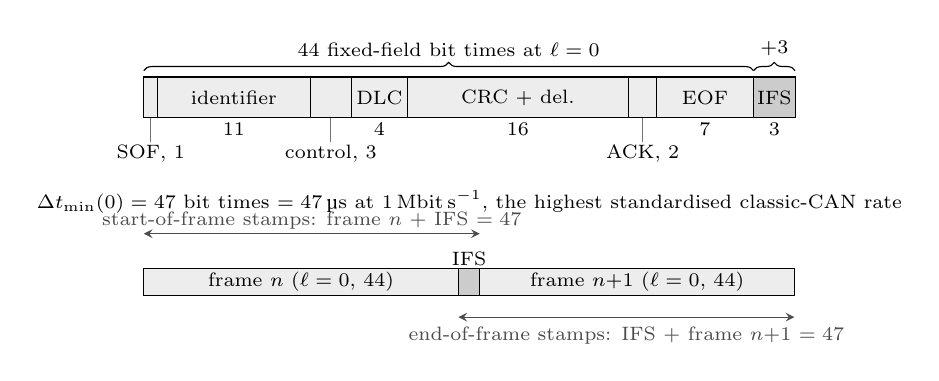
\begin{tikzpicture}[x=0.176cm, y=1cm, font=\scriptsize]

% ---- the frame at l = 0, field by field -------------------------------------------
\foreach \a/\b/\name in {0/1/, 1/12/identifier, 12/15/, 15/19/DLC, 19/35/{CRC $+$ del.},
                         35/37/, 37/44/EOF} {
  \draw[fill=black!7] (\a,0) rectangle (\b,0.52);
  \node[font=\fontsize{6.6}{7.4}\selectfont] at ({(\a+\b)/2},0.26) {\name};
}
\draw[fill=black!20] (44,0) rectangle (47,0.52);
\node[font=\fontsize{6.6}{7.4}\selectfont] at (45.5,0.26) {IFS};

% Narrow fields cannot hold their own name; they get leaders to a lower line.
\foreach \x/\lab in {0.5/{SOF, 1}, 13.5/{control, 3}, 36/{ACK, 2}} {
  \draw[black!55, thin] (\x,0) -- (\x,-0.30);
  \node[font=\fontsize{6.6}{7.4}\selectfont, anchor=north, inner sep=1pt] at (\x,-0.30) {\lab};
}
\foreach \x/\n in {6.5/11, 17/4, 27/16, 40.5/7, 45.5/3} {
  \node[font=\fontsize{6.6}{7.4}\selectfont, anchor=north, inner sep=1.5pt] at (\x,0) {\n};
}

% ---- the two brackets that add up to the bound -------------------------------------
\draw[decorate, decoration={brace, amplitude=3pt}] (0,0.60) -- (44,0.60)
      node[midway, anchor=south, inner sep=5pt, font=\fontsize{6.6}{7.4}\selectfont]
      {44 fixed-field bit times at $\ell=0$};
\draw[decorate, decoration={brace, amplitude=3pt}] (44,0.60) -- (47,0.60)
      node[midway, anchor=south, inner sep=5pt, font=\fontsize{6.6}{7.4}\selectfont] {$+3$};
\node[anchor=north, font=\scriptsize] at (23.5,-0.80)
      {$\dtmin(0)=47$ bit times $=\SI{47}{\micro\second}$ at \SI{1}{\mega\bit\per\second},
       the highest standardised classic-CAN rate};

% ---- why the stamping convention does not matter -----------------------------------
% Drawn to the same bit-time scale as the panel above, just compressed, so the two spans
% come out the same length on the page rather than being asserted equal in a label.
\begin{scope}[yshift=-2.25cm, x=0.0908cm]
  \draw[fill=black!7] (0,0) rectangle (44,0.34);
  \node[font=\fontsize{6.6}{7.4}\selectfont] at (22,0.17) {frame $n$ ($\ell=0$, 44)};
  \draw[fill=black!20] (44,0) rectangle (47,0.34);
  \draw[fill=black!7] (47,0) rectangle (91,0.34);
  \node[font=\fontsize{6.6}{7.4}\selectfont] at (69,0.17) {frame $n{+}1$ ($\ell=0$, 44)};
  \node[font=\fontsize{6.6}{7.4}\selectfont, anchor=south, inner sep=1pt] at (45.5,0.34) {IFS};

  \draw[<->, >=stealth, black!70] (0,0.78) -- (47,0.78)
        node[midway, anchor=south, inner sep=1.5pt, font=\fontsize{6.6}{7.4}\selectfont]
        {start-of-frame stamps: frame $n$ $+$ IFS $=47$};
  \draw[<->, >=stealth, black!70] (44,-0.28) -- (91,-0.28)
        node[midway, anchor=north, inner sep=3.2pt, font=\fontsize{6.6}{7.4}\selectfont]
        {end-of-frame stamps: IFS $+$ frame $n{+}1$ $=47$};
\end{scope}
\end{tikzpicture}

\caption{Where the bound of the nominal floor $\Delta t_{\min}=(47+8\ell)/R$ comes from, at $\ell=0$. The frame's
seven fixed fields sum to 44 bit times and the interframe space adds three: a nominal
47-bit-time lower bound, \SI{47}{\micro\second} at the highest standardised rate of
\SI{1}{\mega\bit\per\second}. The lower panel shows both stamping conventions on a common
bit-time scale: at $\ell=0$ start-of-frame and end-of-frame stamping span the same 47 bit
times, so the bound does not depend on where the logger stamps. Bit stuffing is excluded
because it can only lengthen a frame.}
\label{fig:floor}
\end{figure}
\clearpage
\section*{S2. Audit pseudocode}
\begin{algorithm}[H]
\caption{Exact-arithmetic audit specification for ROAD and can-train-and-test}
\label{alg:audit}
\KwIn{ROAD or can-train-and-test capture files $\mathcal{C}$}
\KwOut{per-file verdict, $\rho_<$, epoch and span flags, per-identifier cross-check}
$\dtmin \leftarrow \SI{47}{\micro\second}$%
  \tcp*{$\Delta t_{\min}=(47+8\ell)/R$ at $R=1$\,Mbit/s, $\ell=0$; 47 or 0.000047 in file units}
\ForEach{file $c \in \mathcal{C}$}{
  parse timestamps exactly as $\hat t_1\dots\hat t_n$: integer microseconds where the log
    has fixed precision, exact decimals otherwise
    \tcp*{exact timestamp-string parsing; can-train-and-test takes the second branch}
  $\gex \leftarrow$ successive differences of $\hat t$, exact in that representation\;
  select eligible gap indices $\mathcal{G}_c$ using the corpus-specific rule above\;
  $\rho_< \leftarrow |\{i\in\mathcal{G}_c:\gex_i < \dtmin\}| / |\mathcal{G}_c|$\;
  $\text{epoch} \leftarrow \ind[\,\hat t_1 \text{ is a whole number of seconds}\,]$\;
  $\text{span} \leftarrow \hat t_n-\hat t_1$, rescaled to seconds; compare with declared duration\;
  \ForEach{identifier $a \in \mathcal{A}(c)$}{
    $\tilde\nu_a \leftarrow \operatorname{median}$ of positive same-identifier intervals
      \tcp*{label-free; not the $\nu_a$ of the main paper\textquotesingle s benign-training nominal period}
    flag $a$ iff $\tilde\nu_a < \dtmin$\;
  }
  verdict $\leftarrow$ \textsc{Timing-reference implausible} \textbf{if} $\rho_< > 0.01$
    \textbf{else} \textsc{Passes this screen}
    \tcp*{empirical screen, not source identification; the main paper\textquotesingle s conclusion}
}
\Return{verdicts}\;
\end{algorithm}
\clearpage
\section*{S3. Damage taxonomy}
\begin{figure}[H]
\centering
% The three damage levels, with the empty one drawn empty.
% No generator: this is the taxonomy of Section 3.3, not a measurement. Only the level
% assignment the text states explicitly (ROAD supports L1; L3 is not identified) appears here; can-train-and-test
% is deliberately absent because the paper never assigns it a level, and inferring one from
% its rho_< would be the figure making a claim the manuscript does not.
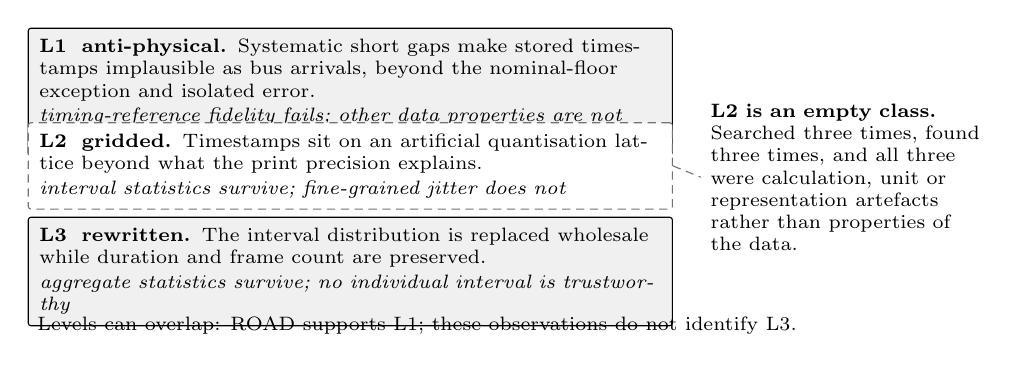
\begin{tikzpicture}[font=\scriptsize, x=1cm, y=1cm]
\tikzset{
  lvl/.style={draw, rounded corners=1pt, minimum height=1.02cm, text width=7.9cm,
              inner sep=4pt, align=left, anchor=north west},
  full/.style={lvl, fill=black!6},
  hollow/.style={lvl, fill=white, densely dashed, draw=black!55},
  tag/.style={font=\fontsize{6.6}{7.4}\selectfont, anchor=north west, inner sep=0pt},
}

\node[full] at (0,0)
  {\textbf{L1 \ anti-physical.} Systematic short gaps make stored timestamps
   implausible as bus arrivals, beyond the nominal-floor exception and isolated error.\\[1pt]
   \textit{\fontsize{6.6}{7.4}\selectfont timing-reference fidelity fails; other data properties are not assessed}};

\node[hollow] (l2box) at (0,-1.20)
  {\textbf{L2 \ gridded.} Timestamps sit on an artificial quantisation lattice beyond
   what the print precision explains.\\[1pt]
   \textit{\fontsize{6.6}{7.4}\selectfont interval statistics survive; fine-grained jitter does not}};

\node[full] at (0,-2.40)
  {\textbf{L3 \ rewritten.} The interval distribution is replaced wholesale while duration
   and frame count are preserved.\\[1pt]
   \textit{\fontsize{6.6}{7.4}\selectfont aggregate statistics survive; no individual interval is trustworthy}};

% The empty class is the result, so it is marked on the figure rather than left to the text.
\node[anchor=west, font=\scriptsize, align=left, text width=3.5cm] (l2note)
     at (8.55,-1.90)
     {\textbf{L2 is an empty class.}\\ Searched three times,
      found three times, and all three were calculation, unit or representation artefacts
      rather than properties of the data.};
% 锚定到节点边缘，不手算坐标：旧线画在 (7.95)-(8.1)，两端都落在 L2 框内部。
\draw[black!55, densely dashed] (l2box.east) -- (l2note.west);

\node[anchor=north west, font=\scriptsize, align=left] at (0,-3.55)
  {Levels can overlap: ROAD supports L1; these observations do not identify L3.};
\end{tikzpicture}

\caption{The three damage levels of the main paper\textquotesingle s taxonomy. The italic line in
each box states what that level leaves usable and what it destroys; the three differ,
which is why ``synthetic'' alone does not tell a practitioner which uses are affected.
L2 is drawn dashed and empty because no genuine instance appears in the four corpora
audited here---a result, not an unfinished search.}
\label{fig:taxonomy}
\end{figure}
\clearpage
\section*{S4. Published statements and measurements}
\begin{table}[H]
\centering
\caption{Documented timestamp handling in ROAD against measurement. The last row is the
authors' own methodological position, applied to a different corpus.}
\label{tab:official}
\begin{tabular}{>{\raggedright\arraybackslash}p{0.44\linewidth}>{\raggedright\arraybackslash}p{0.44\linewidth}}
\toprule
Published statement & Measurement \\
\midrule
``Absolute timestamps are shifted uniformly by a scalar'' \citep{road,roadzenodo} &
A constant shift preserves all gaps. Observed: sub-floor gaps and integer-second starts in 45/45 files. \\
\addlinespace
Timestamps ``are reported with a precision of \SI{1}{\micro\second}'', while the capture
hardware ``only guarantees an accuracy of \SI{100}{\micro\second}'' \citep{road,roadzenodo} &
Stated accuracy alone does not explain sub-floor gaps at a \SI{1}{\micro\second} median; print precision is not a capture-time error model. \\
\addlinespace
Masquerade captures are ``slightly modified in post-processing'' by ``removing the
legitimate target ID frames preceding each injected frame'' \citep{road} &
Frame removal merges gaps, creates none; ambient captures, uncovered by any modification statement, carry the same signature. \\
\addlinespace
``Adjusting timestamps in post-processing alters data and diminishes fidelity in a
critical way'' \citep{road} &
The authors' own criterion, stated when assessing a different corpus. \\
\bottomrule
\end{tabular}
\end{table}
\clearpage
\section*{S5. Current and historical sensitivity evidence}
The current complete run contains 58 evaluation files, 141 configurations per file and
8178 result rows. The corrected SynCAN reader retains the first normal frame of each
of three headerless training files. Stored metrics change in 610 SynCAN rows relative
to the historical result; unknown historical code, input and cache identities prevent
attribution solely to the three restored rows. The new run replaces those sensitivity
estimates; it does not retrospectively certify the historical runtime. The CTAT and ROAD
groups contain 40 and 13 evaluation files, and SynCAN contributes five attack test files;
its separate baseline also includes the normal test file. The main paper reports each
numeric estimand with its population and precision.
\bibliographystyle{IEEEtranN}
\bibliography{references}
\end{document}
